\section{Web Tabanlı Konteyner Orkestrasyon Sistemi}\label{sec:study}
Bu çalışma, kullanıcıların konteyner teknolojilerini kullanarak konteynerlerle etkileşimde bulunmasını sağlayan bir web arayüzü sağlar. Çalışma, kullanıcıların hazırlanan bir formu doldurarak konteyner oluşturma, çalıştırma ve konteynerden gelen çıktıları grafik ve tablo şeklinde elde etme imkanı sunar.\\
Ayrıca, çalışmanın kullanıcı arayüzü ve arkaplan (backend) işleyişi hakkında da bilgi verilmektedir.
\subsection{Kullanıcı Arayüz}
Kullanıcı arayüzü, özel bir template seçilerek çalışmanın gereksinimlerine uygun hale getirilmiştir. Template içerisinde gereksiz kısımlar temizlenerek sağ menü bölümü oluşturulmuştur. Bu sayede kullanıcılar, sağ menü üzerinden kolayca erişebilecekleri Dashboard, görevler (Ping, Theharvester), sistem kayıtları ve Profil gibi önemli bölümlere ulaşabilmektedir. Bu düzenlemeler, arayüzün kullanıcı dostu ve çalışmaya özgü bir hale gelmesini sağlamaktadır.

\textbf{Oturum Açma} : Kullanıcıların uygulamayı kullanabilmek için oturum açmalarını sağlar. Kullanıcı, kayıtlı e-posta adresi ve şifresini girerek oturum açma işlemini gerçekleştirir.
\begin{figure}[ht]
	\centering
	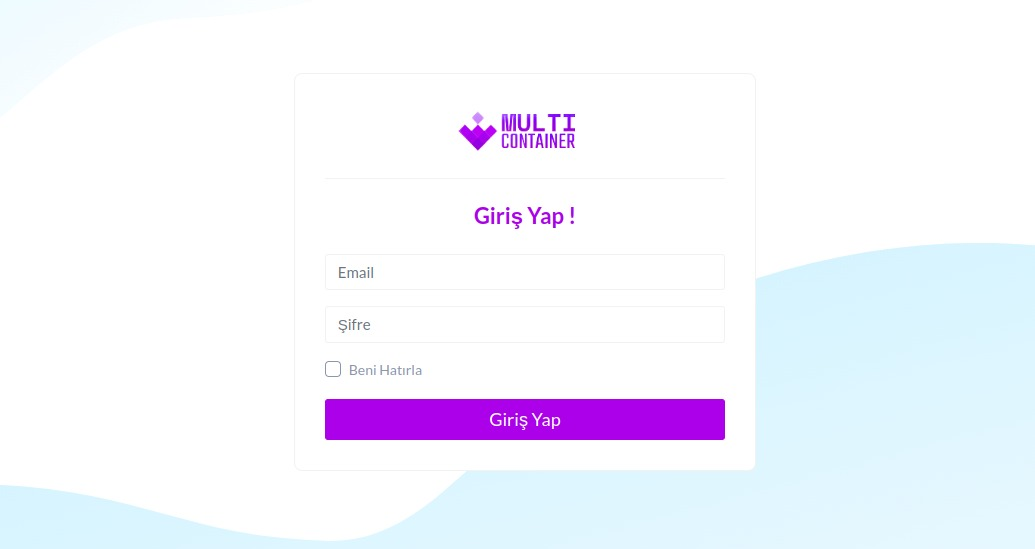
\includegraphics[width=0.9\linewidth]{images/login.jpeg}
	\caption{Giriş sayfası}
	\label{fig:login}
\end{figure}

Şekil \ref{fig:login}'de görüldüğü gibi oturum açma sayfası, kullanıcıya e-posta ve şifre alanlarını doldurarak oturum açma imkanı sunar. Kullanıcının girdiği e-posta adresi ve şifre, kayıtlı bilgilerle doğrulandıktan sonra oturum açma işlemi tamamlanır.

Kullanıcı oturumu başarıyla açtığında, \textbf{Kontrol Paneli} sayfasıyla karşılaşacaktır. Şekil \ref{fig:dashboard}'de görüldüğü gibi, bu sayfa kullanıcıya genel bir bakış sağlar ve Ping ve Theharvester konteynerlerine ilişkin istatistikleri grafik ve tablo şeklinde sunar.

\begin{figure}[ht]
	\centering
	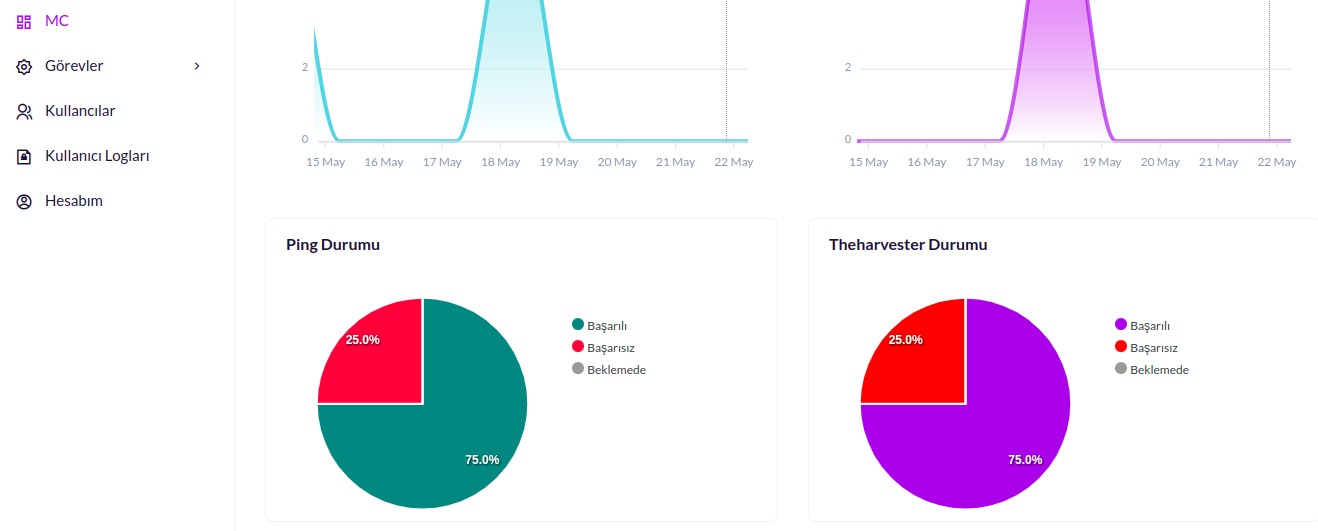
\includegraphics[width=0.9\linewidth]{images/dashboard.jpeg}
	\caption{Kontrol paneli sayfası}
	\label{fig:dashboard}
\end{figure}

Kontrol Paneli sayfasında kullanıcı, Ping ve Theharvester konteynerlerine ait verileri kolayca görüntüleyebilir. İlk olarak, kullanıcının sahip olduğu konteynerlerin sayısı bir grafikle gösterilir. Bu grafik, belirli bir zaman diliminde kullanıcının konteynerlerinin değişimini görsel olarak sunar.

Ardından, Ping ve Theharvester görevlerinin istatistikleri gösterilir. Kullanıcı, başarılı, başarısız ve beklemede olan görevlerin sayısını görüntüleyebilir. Bu bilgi, kullanıcının görevlerinin durumunu hızlıca anlamasına yardımcı olur.

Sayfanın alt kısmında, en son 5 görev tablo şeklinde listelenir. Bu liste, kullanıcının en son gerçekleştirdiği görevleri ve ilgili bilgileri içerir. Kullanıcılar, bu tablo üzerinden son görevlerini takip edebilir ve detaylı bilgilere erişebilir.

Kontrol Paneli sayfası, kullanıcıların konteynerlerine ilişkin genel bir bakış elde etmelerini ve önemli istatistikleri görsel ve tablo şeklinde görüntülemelerini sağlar. Bu sayede kullanıcılar, uygulamanın sağladığı konteyner orkestrasyon sisteminin performansını hızlıca değerlendirebilirler.

Panelden yeni görevler oluşturmak için \textbf{Ping Oluşturma Sayfası} kullanılır. Şekil \ref{fig:create}'te gösterilen form, kullanıcının Ping görevlerini oluşturmasını sağlar.

\begin{figure}[ht]
	\centering
	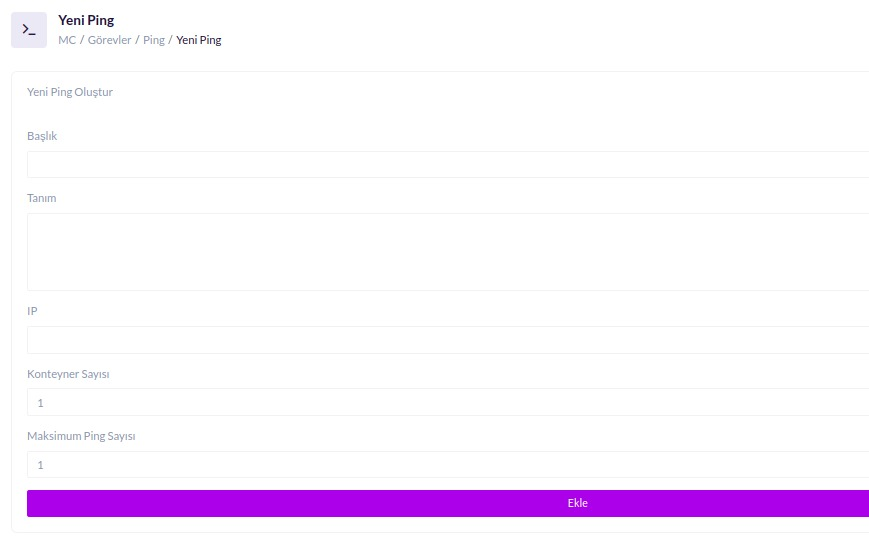
\includegraphics[width=0.9\linewidth]{images/create.jpeg}
	\caption{Ping oluşturma sayfası}
	\label{fig:create}
\end{figure}

Formda, kullanıcıdan aşağıdaki bilgileri girmesi istenir:
\begin{itemize}
	\item Görev Başlığı: Oluşturulacak görevin başlığı.
	\item Açıklama: Görevle ilgili detaylı açıklama.
	\item Ping IP Adresi: Ping işleminin gerçekleştirileceği hedef IP adresi.
	\item Ping Sayısı: Kaç adet ping atılacağı.
	\item Konteyner Sayısı: Bu görevi gerçekleştirecek konteynerlerin sayısı.
\end{itemize}

Bu bilgilerin tamamı zorunlu alanlardır ve kullanıcı tarafından doldurulması gerekmektedir. Kullanıcılar, bu formu doldurarak yeni Ping görevleri oluşturabilir ve bu görevlerin konteynerler tarafından gerçekleştirilmesini sağlayabilir.

Ping Oluşturma Sayfası, kullanıcılara kolay ve kullanıcı dostu bir şekilde yeni görevler oluşturma imkanı sunar. Kullanıcılar, bu form üzerinden gerekli bilgileri girerek istedikleri Ping görevini tanımlayabilir ve uygulamanın konteynerler aracılığıyla bu görevi gerçekleştirmesini sağlayabilirler.

Oluşturulan Ping görevleri, \textbf{Ping Görev Listesi} adı verilen bir tablo şeklinde görüntülenir. Şekil\ref{fig:ping_list}'de gösterilen tabloda, her görevin aşağıdaki bilgileri listelenir:

\begin{itemize}
	\item Görev Başlığı: Oluşturulan görevin başlığı.
	\item konteyner: Oluşturulan konteyner sayısı.
	\item Oluşturan: Görevin kimin tarafından oluşturuldu
	\item Durumu: Görevin mevcut durumu, başlangıçta "Beklemede" olarak gösterilir.
	\item Görev Oluşturma Tarihi
	\item Detay Botunu: Görev detayı görüntülebilmektir
\end{itemize}

\begin{figure}[ht]
	\centering
	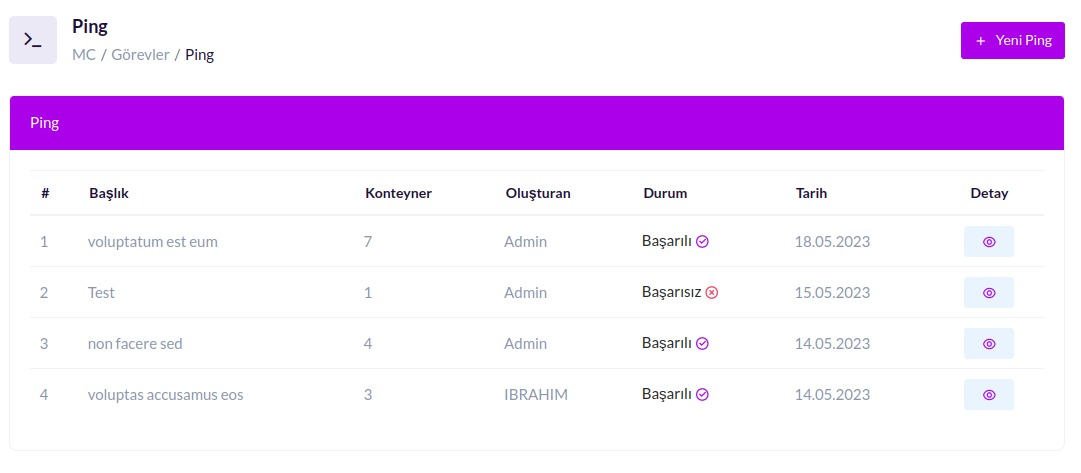
\includegraphics[width=0.9\linewidth]{images/ping_list.jpeg}
	\caption{Ping görev listesi}
	\label{fig:ping_list}
\end{figure}

Görevlerin işlem durumu tamamlandığında, kullanıcılar detaylarına erişebilir. Görev detayı aşağıdaki bölümlerden oluşur:
\begin{itemize}
	\item Konteyner Grafikleri: Görevin çalıştırıldığı konteyner sayısına göre grafikler oluşturulur. Her grafikte, minimum, ortalama, maksimum ping değerleri ve ping kaybı gösterilir. Şekil\ref{fig:container_graphic}'de bu grafiklerin bir örneği görülebilir.
	      \begin{figure}[ht]
		      \centering
		      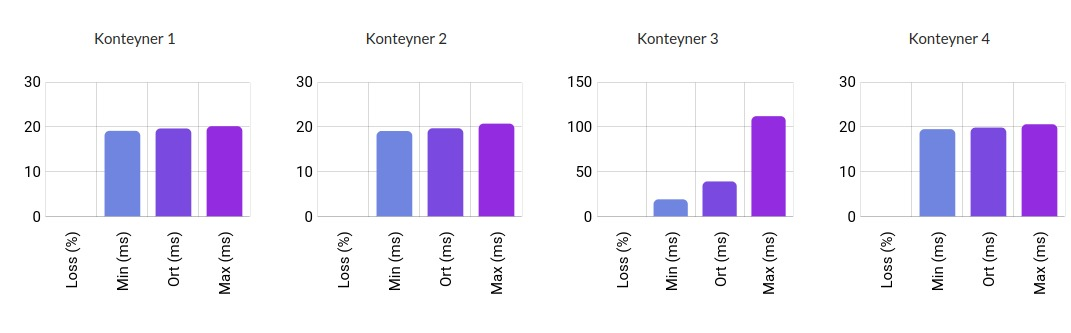
\includegraphics[width=0.9\linewidth]{images/ping_graphic.jpeg}
		      \caption{konteyner grafikleri}
		      \label{fig:container_graphic}
	      \end{figure}

	\item Görev Detayı: Görevin genel detayları, başlığı, açıklaması, atılan ping IP adresi, ping sayısı ve kullanılan konteyner sayısı gibi bilgiler içerir. Şekil\ref{fig:ping_detail}'de bu detayların bir örneği görülebilir.
	      \begin{figure}[ht]
		      \centering
		      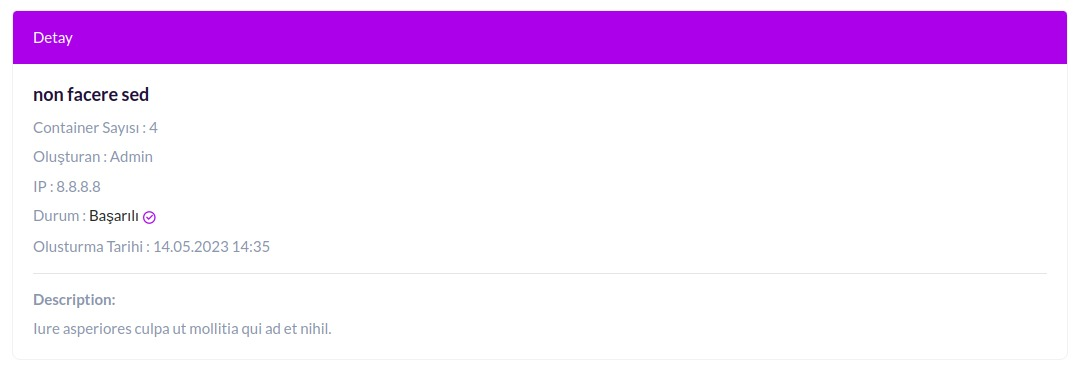
\includegraphics[width=0.9\linewidth]{images/ping_detail.jpeg}
		      \caption{Ping görev detayı}
		      \label{fig:ping_detail}
	      \end{figure}

	\item Konteyner Detayları ve Çıktıları: Görevin çalıştırıldığı konteynerlerin ayrıntıları ve çıktıları bu bölümde görüntülenir. Konteynerlerin detaylarını içeren bir tablo ve her konteynerin çıktılarını gösteren ayrı bir tablo bulunur. Şekil \ref{fig:container_detail} ve şekil \ref{fig:container_output}'de bu detayların örneklerini gösterir.
	      \begin{figure}[ht]
		      \centering
		      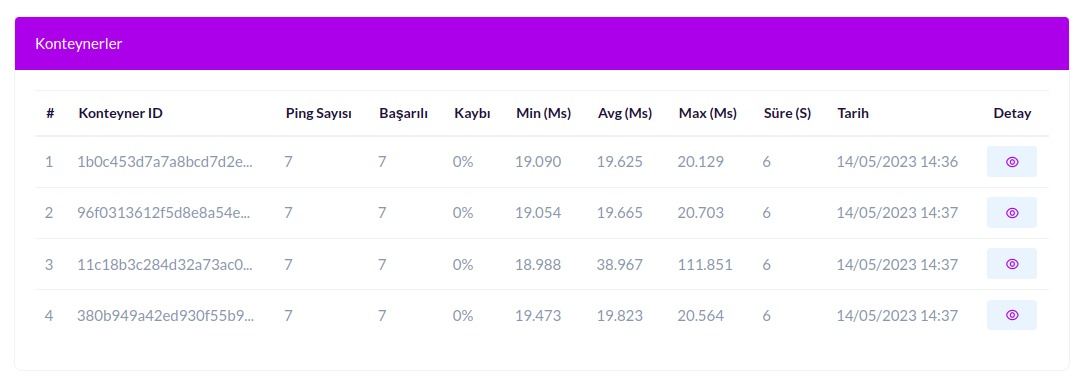
\includegraphics[width=0.9\linewidth]{images/container_detail.jpeg}
		      \caption{Konteyner detayı}
		      \label{fig:container_detail}
	      \end{figure}

	      \begin{figure}[ht]
		      \centering
		      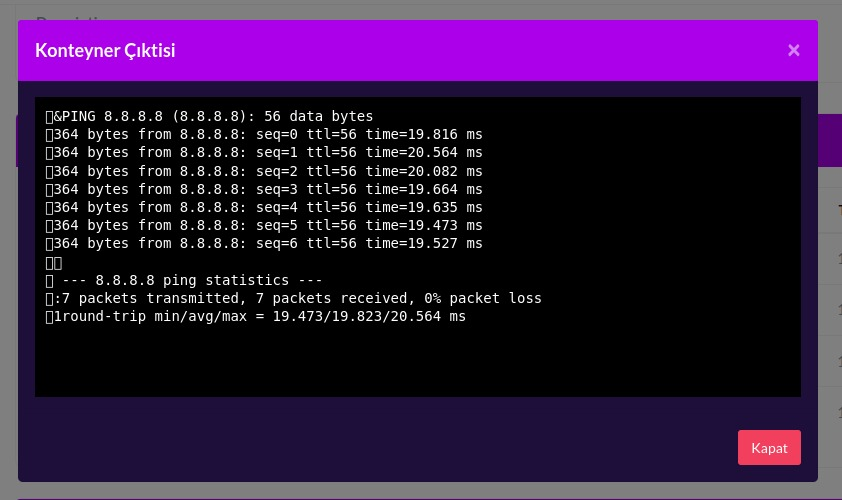
\includegraphics[width=0.9\linewidth]{images/container_output.jpeg}
		      \caption{Konteyner çıktısı}
		      \label{fig:container_output}
	      \end{figure}
	\item Görev sırasında oluşan hatalar bu tabloda listelenir. Her hata, hata mesajı ve hatanın oluştuğu konteyner bilgileriyle birlikte gösterilir. Şekil \ref{fig:container_error}'de bu hata listesinin bir örneği görülebilir.
	      \begin{figure}[ht]
		      \centering
		      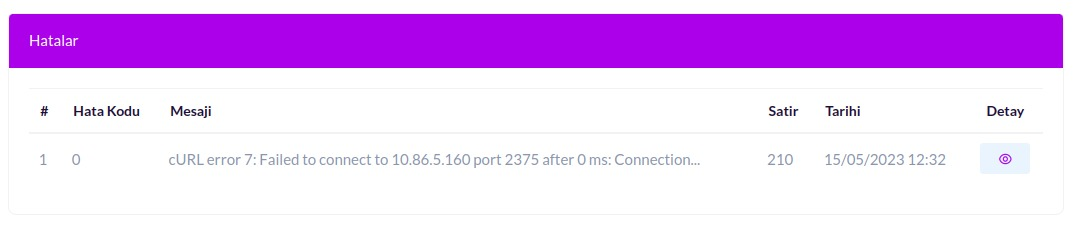
\includegraphics[width=0.9\linewidth]{images/container_error.jpeg}
		      \caption{Konteyner hataları}
		      \label{fig:container_error}
	      \end{figure}
\end{itemize}

Bu görev detayları, kullanıcılara görevlerin ayrıntılı bilgilerini, konteyner performansını, çıktıları ve oluşan hataları inceleme imkanı sunar. Kullanıcılar, bu detaylar sayesinde görevlerin çalışma durumunu, konteynerlerin performansını ve olası sorunları kolayca analiz edebilirler.

\textbf{Kullanıcılar} bölümünde, kullanıcıların oluşturulması, görüntülenmesi, güncellenmesi ve silinmesi gibi işlemler gerçekleştirilebilir. Şekil \ref{fig:users}'de, \textbf{Kullanıcılar Listesi} adı verilen bir tablo şeklinde kullanıcıların listelendiği görülmektedir.

Her kullanıcı için aşağıdaki bilgiler listelenir:
\begin{itemize}
	\item Kullanıcı Adı ve Soyadı.
	\item E-posta: Kullanıcının kayıtlı e-posta adresi.
	\item Oluşturma Tarihi: Kullanıcının oluşturulma tarihi.
	\item İşlem sütunuda mevcuttur.
\end{itemize}

Bu tablo, sisteme kayıtlı olan tüm kullanıcıların genel bilgilerini görüntüler. Kullanıcılar, bu tablo üzerinden kullanıcıları inceleyebilir, güncelleyebilir veya silme işlemleri gerçekleştirebilir. Bu sayede sistem yöneticileri, kullanıcılarla ilgili işlemleri kolaylıkla yapabilir ve kullanıcı verilerini yönetebilir.
\begin{figure}[ht]
	\centering
	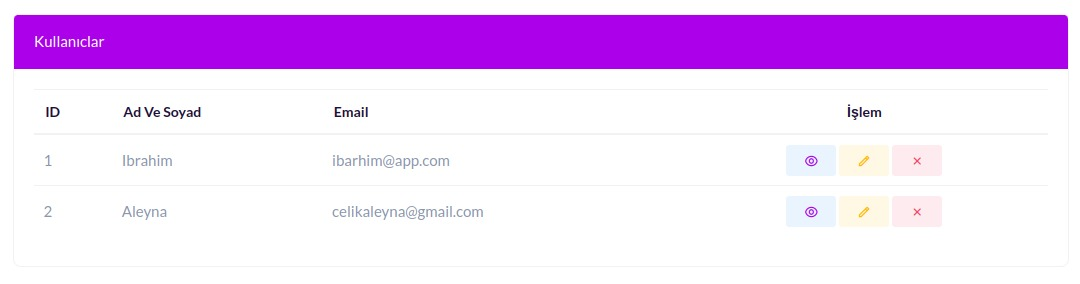
\includegraphics[width=0.9\linewidth]{images/users.jpeg}
	\caption{Kullanıcılar listesi}
	\label{fig:users}
\end{figure}

\textbf{Kullanıcı kayıtları} bölümünde, her kullanıcının yaptığı aktivitelerin bir log listesi olarak görüntülendiği bir tablo bulunmaktadır. Şekil \ref{fig:log}'de, Kullanıcı kayıtları tablosu örneği gösterilmektedir.
Bu tabloda her log girdisi için aşağıdaki bilgiler listelenir:
\begin{itemize}
	\item Kullanıcı: İlgili kullanıcının adı ve Soyadı.
	\item IP: Kullanıcının oturum açtığı IP adresi.
	\item İşlem: Kullanıcının gerçekleştirdiği işlem veya aktivite açıklaması.
	\item Tarih: İşlemin gerçekleştiği tarih.
	\item Saat: İşlemin gerçekleştiği saat.
\end{itemize}

\begin{figure}[ht]
	\centering
	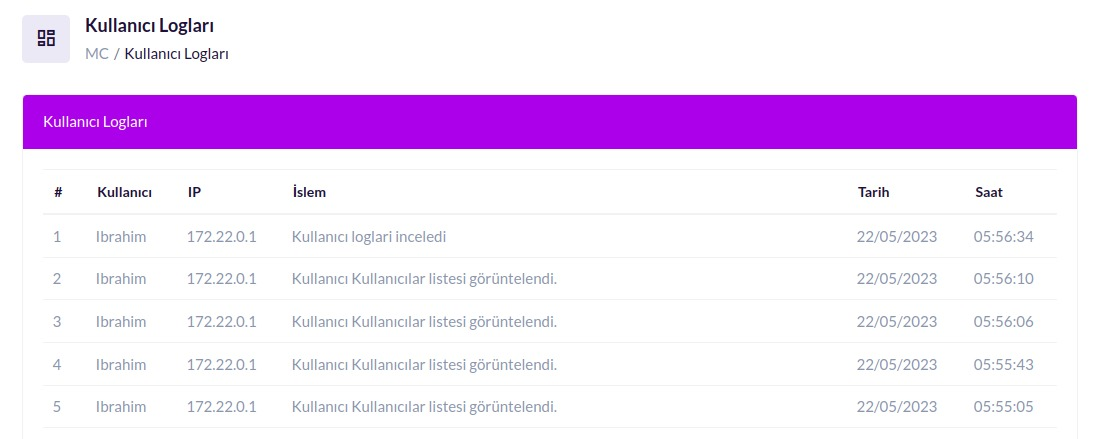
\includegraphics[width=0.9\linewidth]{images/log.jpeg}
	\caption{Kullanıcı kayıtları}
	\label{fig:log}
\end{figure}

Bu kayıtlar, kullanıcı aktivitelerinin izlenmesi, takibi ve güvenlik amaçlı olarak kullanılabilir. Sistem yöneticileri veya yetkilileri, bu kayıtları kullanarak kullanıcıların yaptığı işlemleri inceleyebilir ve gerekirse uygun önlemleri alabilir. Ayrıca, kullanıcı kayıtları, sistemdeki kullanıcı etkinliği hakkında bilgi sahibi olmak için kullanılabilir.
\textbf{Hesabım} bölümünde, oturum açmış olan kullanıcının kendi hesap bilgilerini güncelleyebileceği bir form bulunmaktadır. Şekil \ref{fig:account}'de, "Oturum açan kullanıcı hesabı" formu örneği gösterilmektedir.
\begin{figure}[ht]
	\centering
	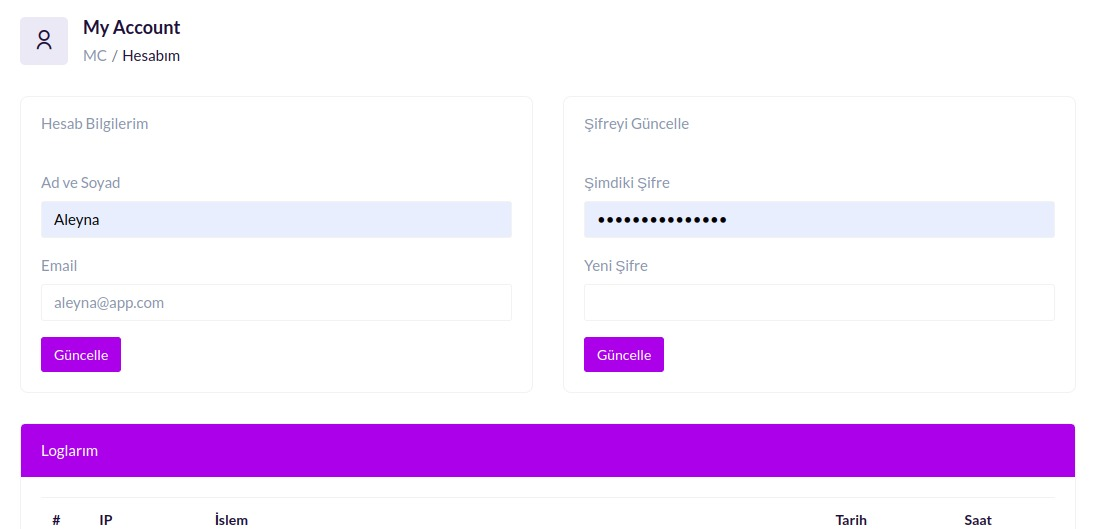
\includegraphics[width=0.9\linewidth]{images/account.jpeg}
	\caption{Oturum açan kullanıcı hesabı}
	\label{fig:account}
\end{figure}

Ayrıca, kullanıcının kendi kayıtları da tablo şeklinde görüntülenmektedir. Bu kayıtlar, kullanıcının kendi aktivitelerini takip etmek ve geçmiş işlemlerini gözden geçirmek için kullanılabilir.

\subsection{Arkaplanda Çalışan Servisler (Backend)}

Daha önce \ref{subsec:docker} bölümünde bahsettiğimiz gibi, Docker Engine PHP özelliğini kullanarak Laravel uygulamasıyla iletişim sağlayan "PingService" adında bir servis geliştirilmiştir. Bu servis sayesinde konteyner oluşturma, çalıştırma, detaylarını görüntüleme gibi işlemler gerçekleştirilebilir.

Konteyner oluşturmak için Docker Engine API'sini kullanarak POST metoduyla \\ \textbf{https://example.com/v14/containers/create}  adresine bir istek atılması gerekmektedir. İstek gövdesi (body) iki parametre içermektedir:
\begin{itemize}
	\item Image: Hangi imajın kullanılacağı
	\item Cmd: Hangi komutun çalıştırılacağı
\end{itemize}

Bu parametreler, JSON formatında gönderilmektedir.

Aşağıda, bir ping görevi oluşturma örneği verilmiştir:

\begin{lstlisting}[language=PHP]
  $response = $this->client->post('/containers/create', [
  'json' => [
  'Image' => 'alpine',
  'Cmd' => ['ping', '-c', $this->ping->max_ping, $this->ping->ip]
  ]
  ]);
  \end{lstlisting}

Bu örnek, \textbf{alpine} imajını kullanarak \textbf{ping} komutunu belirtilen parametrelerle çalıştırmak için bir konteyner oluşturur.

\say{ Alpine, hafif ve güvenli bir Linux dağıtımıdır. Docker tarafından resmi olarak desteklenen ve sıkça kullanılan bir imajdır. Alpine, minimal bir yapıya sahiptir ve gereksiz bileşenleri içermez, bu nedenle küçük boyutlu ve hızlı çalışan konteynerler oluşturmak için tercih edilir \cite{alpine}.}

İşte belirli bir işlem için oluşturulan konteynerin geri döndürdüğü JSON yanıtını kullanarak konteyner kimliğini ve uyarıları elde etmek için PHP kodu:

\begin{lstlisting}[language=PHP]
	$responseJson = '{
	  "Id": "a468317ac3533ff0dde4857bb7e50c51953293073e9ae5975e7cb5a114b8463a",
	  "Warnings": []
	}';
	
	$responseArray = json_decode($responseJson, true);
	$containerId = $responseArray['Id'];
	$warnings = $responseArray['Warnings'];
\end{lstlisting}

Bu kod, JSON yanıtını doğru bir şekilde bir PHP dizisine dönüştürür. Ardından, konteyner kimliğini (\texttt{\$containerId}) ve uyarıları (\texttt{\$warnings}) ilgili değişkenlere atar.

Daha sonra, elde edilen konteyner kimliğiyle yapılacak işlemleri gerçekleştirebilirsiniz. Örneğin:

\begin{lstlisting}[language=PHP]
	
	$this->startContainer($containerId);
	
	$this->stopContainer($containerId);
	
	$this->getContainerLogs($containerId);
	
	$this->storeContainerLogs($parsedLogs, $containerId, $operation_time);
\end{lstlisting}

Bu kod parçacığı, belirli bir işlemi gerçekleştirmek için konteyner kimliğini kullanılması olanak sağlar. İlgili işlemler \textbf{startContainer}, \textbf{stopContainer}, \textbf{getContainerLogs} ve \textbf{storeContainerLogs} olarak adlandırılan fonksiyonlar özel olarak yazılmıştır.

Aşağıda, Docker Engine API ile Laravel'in nasıl bağlandığını gösteren PHP kodu yer almaktadır. Bu kod, guzzle\cite{guzzle_documentation} kütüphanesini kullanarak Docker Engine API'ye bağlantı sağlamaktadır. `Ping` sınıfı bağımlılığı da burada enjekte edilmektedir.
nd{figure}

\begin{lstlisting}[language=PHP, caption={Ping sınıfının yapıcısı}, label={lst:ping_construct}]
	public function __construct(public Ping $ping)
	{
		$this->logger = Log::channel('single');
		
		try {
			$this->client = new Client([
				'base_uri' => config('services.docker.endpoint'),
				'timeout' => config('services.docker.timeout')
			]);
		} catch (\Exception $e) {
			$this->saveEventualErrors($e);
			$this->logger->error($e->getMessage());
		}
	}
	\end{lstlisting}
	


Şekil \ref{lst:ping_construct}'deki kodda, Docker Engine API'ye bağlantı sağlamak için `Client` sınıfı oluşturulmaktadır. `base uri` parametresi, Docker API endpointini belirtmektedir ve `timeout` parametresi, API çağrılarının zaman aşımı süresini belirlemektedir. Oluşturulan `Client` nesnesi, sınıfın diğer metotlarında kullanılmak üzere `this->client` değişkenine atanmaktadır.

Hata durumunda, `try-catch` bloğu kullanılarak hata yakalanmakta ve ilgili işlemler gerçekleştirilmektedir. Hata durumunda, hata kaydedilip gerekli kayıt alma işlemleri yapılmaktadır.

Şekil \ref{lst:ping_func}'deki kodda, createPingContainer fonksiyonunu içerir. İlk olarak, IP adresinin doğruluğu kontrol edilir ve geçerli değilse bir hata fırlatılır. Daha sonra, mevcut konteynerleri siler.

Döngü kullanarak, belirli sayıda ping konteyneri oluşturulur. Her konteyner oluşturulduğunda, Docker API'ye bir POST isteği gönderilir ve konteyner oluşturulur. Oluşturulan konteyner başlatılır ve belirli bir süre (burada 10 saniye) beklenir. Ardından konteyner durdurulur.

Konteynerin çalışma süresi ve kayıtları elde edilir ve ilgili işlemler gerçekleştirilir. Son olarak, ping nesnesinin durum güncellemesi yapılır ve ilgili kayıt alma işlemleri gerçekleştirilir.

Hata durumunda, hata yakalanır, gerekli işlemler gerçekleştirilir ve hata mesajı kayıt edilir.

Bu şekilde, createPingContainer fonksiyonu, ping görevi için gerekli konteynerleri oluşturur ve ilgili işlemleri gerçekleştirir.

\begin{lstlisting}[language=PHP, caption={Ping görevi servis metodu}, label={lst:ping_func}]
	public function createPingContainer(): void
    {
        // Validate the IP address
        if (!filter_var($this->ping->ip, FILTER_VALIDATE_IP)) {
            throw new \InvalidArgumentException('Invalid IP address: ' . $this->ping->ip);
        }
        $this->ping->containers()->delete();
        
        try {
            $this->logger->info('start creating container');
            for ($i = 0; $i < $this->ping->container; $i++) {     // Create the container
                $response = $this->client->post('/containers/create', [
                    'json' => [
                        'Image' => 'alpine',
                        'Cmd' => ['ping', '-c', $this->ping->max_ping, $this->ping->ip]
                    ]
                ]);
                
                $container = json_decode((string)$response->getBody(), true);
                
                // Start the container
                $this->logger->info('Started container with ID: ' . $container['Id']);
                $this->startContainer($container['Id']);
                
                
                Sleep::for(10)->seconds();
                
                $this->stopContainer($container['Id']);
                
                $operation_time = $this->containerRunTime($container['Id']);
                
                $logs = $this->getContainerLogs($container['Id']);
                
                $parsedLogs = $this->parseContainerLogs($logs);
                
                $this->storeContainerLogs($parsedLogs, $container['Id'], $operation_time);
            }
            $this->ping->update(['status' => 1]);
            
            $this->logger->info('container is created');
        } catch (\Exception $e) {
            $this->saveEventualErrors($e);
            $this->logger->error($e->getMessage());
        }
    }
	\end{lstlisting}
Konteynerden komut çıktısı alma işlemi şekil \ref{lst:container_cmd_output} gibi gerçekleştirilmektedir:

\begin{lstlisting}[language=PHP, caption={Ping görevi servis metodu}, label={lst:container_cmd_output}]
	public function getContainerLogs(string $containerId): string
    {
        try {
            // Stream the container logs (include both stdout and stderr)
            $response = $this->client->get('/containers/' . $containerId . '/logs?stdout=1&stderr=1&follow=1');
            $stream = $response->getBody();
            
            // Read the logs until the stream is closed
            $logs = '';
            while (!$stream->eof()) {
                $logs .= $stream->read(1024);
            }
            
            return $logs;
        } catch (\Exception $e) {
            $this->logger->error($e->getMessage());
            return '';
        }
    }
	\end{lstlisting}

Konteyner çıktısının parse edilme işlemi şekil \ref{lst:container_parse} gibi yapılmaktadır:

\begin{lstlisting}[language=PHP, caption={Konteyner çıktısı parse işlemi}, label={lst:container_parse}]
	protected function parseContainerLogs(string $log): array
    {
        $data = [
            'packets_transmitted' => '',
            'packets_received' => '',
            'packet_loss' => '',
            'min' => '',
            'avg' => '',
            'max' => '',
            'log' => $log
        ];
        
        preg_match('/(\d+) packets transmitted, (\d+) packets received, (\d+)% packet loss/', $log, $results);
        if (isset($results)) {
            $data['packet_loss'] = $results[3] ?? '';
            $data['packets_transmitted'] = $results[1] ?? '';
            $data['packets_received'] = $results[2] ?? '0';
        }
        
        preg_match('/(\d+\.\d+)\/(\d+\.\d+)\/(\d+\.\d+)/', $log, $matches);
        if (isset($matches)) {
            $data['min'] = $matches[1] ?? '0';
            $data['avg'] = $matches[2] ?? '0';
            $data['max'] = $matches[3] ?? '0';
        }
        
        return $data;
    }
	\end{lstlisting}

Bu şekilde, Docker Engine API ile Laravel arasında bağlantı sağlanmakta ve ping görevi için ilgili fonksiyonlar kullanılmaktadır.

Bir Ping görevi işlem akış diyagramı Şekil çizilmiştir.
\begin{figure}[H]
	\centering
	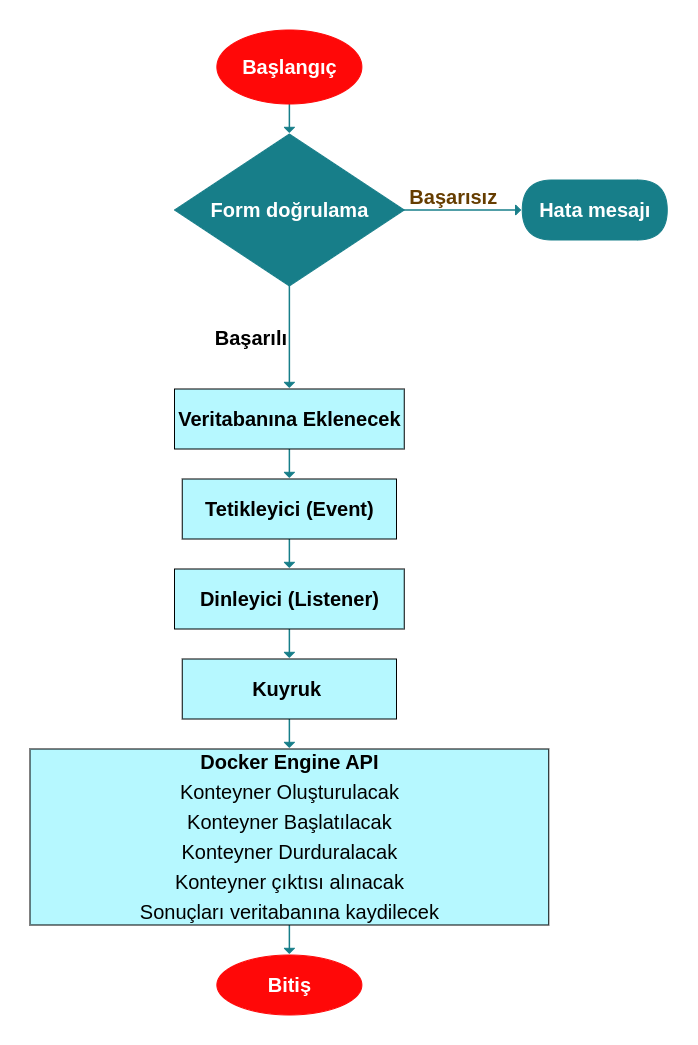
\includegraphics[width=0.9\linewidth]{images/flowchart4.png}
	\caption{Ping görevi çalışma şeması}
	\label{fig:ping_task_diagram}
\end{figure}

\newpage
Bir servis çalışma sureci şekilde gösterilmiştir
\begin{figure}[H]
	\centering
	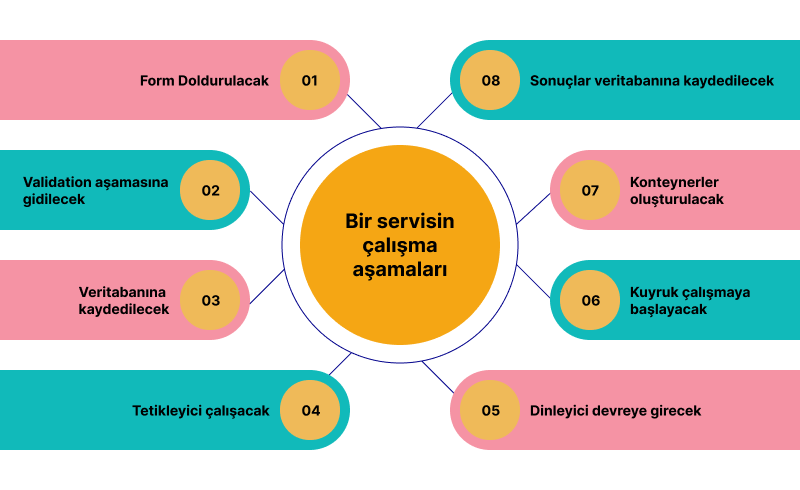
\includegraphics[width=1\linewidth]{images/service.png}
	\caption{Bir görevi çalışma şeması}
	\label{fig:task_diagram}
\end{figure}

\subsection{Uygulamada Servis Ekleme İşlemi}

Bu çalışmada, varsayılan olarak Ping görevi servisi bulunmaktadır. Ekstra servisler eklemek için Laravel paketleri geliştirebilir ve bu paketleri Composer aracılığıyla çalışmaya dahil edilebilir. Örneğin, Theharvester servisi geliştirilmiş ve çalışmaya eklenmiştir.

Theharvester servisini çalışmaya dahil etmek için aşağıdaki adımlar takip edildi:

1. Terminalde çalışmanın bulunduğu dizine aşağıdaki komut kullanıldı:
\begin{lstlisting}[language=bash]
	$ composer require ikay/theharvester-service
\end{lstlisting}

Bu komut, Theharvester servisini çalışmaya Composer aracılığıyla ekleyecektir. Composer, bağımlılıkları otomatik olarak yönetir ve paketi çalışmaya kurar.

2. Son olarak, paketin sağladığı komutları kullanabilmek için çalışmanın yeniden yüklenmesi gerekmektedir. Terminalde aşağıdaki komut çalıştırıldı:
\begin{lstlisting}[language=bash]
	$ php artisan theharvester:install
\end{lstlisting}

Bu komut, Theharvester paketinin bu çalışmada gereken yapılandırmalarını yapacaktır.

Böylece Theharvester servisi çalışmayı başarıyla dahil edilmiş olacaktır. Servisi kullanmaya başlamak için paketin sağladığı komutları veya yöntemleri kullanılabilir. çalışmanın ihtiyaçlarına göre bu yöntemler özelleştirilebilir.

Not : Yukarıdaki adımlar varsayılan bir senaryo üzerinde örneklenmiştir. Paketinizin yapısına ve gereksinimlerine göre adımları uyarlamayı unutmayın.

Theharvester açık kaynak olarak geliştirilmiştir bu github linkinden ulaşabilmektedir : \href{https://github.com/ikhalilatteib/theharvester-service}{https://github.com/ikhalilatteib/theharvester-service}
